% !Mode:: "TeX:UTF-8"
%%% Local Variables:
%%% mode: latex
%%% TeX-master: t
%%% End:

\chapter{引言}
\label{chap:introduction}

\section{研究背景}

动物行为学是生物学研究中一个重要的方向\cite{book_animal_behavior}。动物的行为受到遗传因素和环境因素的影响,而动物行为学通过观察动物的行为研究遗传因素或环境因素对动物的影响。通过动物行为的研究,可以得到一系列有意义的实验成果。其中,比较著名的动物行为学实验包括巴甫洛夫和狗的反射实验\cite{conditional_reflexes}等。

果蝇是动物行为研究中常见的模式生物。首先,果蝇的基因结构简单,目前已有对果蝇基因比较完整的测序,便于生物学家对果蝇基因的操作\cite{tweedie2009flybase};其次,果蝇的身体结构比较简单,便于观察\cite{dankert2009automated}。以上特点使得果蝇在动物行为学中被广泛研究。

但是,动物行为学对动物的观察往往涉及到对大量动物的行为进行观察、计数,上述操作需要大量的人力,往往限制了动物行为学的发展。此外,人工标定动物的行为也往往存在标准不统一、存在主观性等问题\cite{dankert2009automated}。随着计算机视觉和机器学习的发展\cite{chen2015handbook},以及计算机计算能力的提升,使用计算机自动化的分析动物行为成为可能。果蝇身体结构简单,又进一步降低了果蝇自动化分析的难度。计算机对果蝇行为的分析可以大幅度的减少人工识别果蝇行为的工作量,并降低不同视频之间评判标准的差异,对促进果蝇行为学研究有重要的意义。

目前,国内外存在很多果蝇研究小组,如国内有北京大学饶毅教授实验室等\cite{zhou2008subset,liu2011social},国外有Dankert实验室等\cite{dankert2009automated}。不同实验室之间果蝇活动台标准不统一、拍摄设备和光照条件复杂,使得果蝇行为视频分析算法往往只能适配单独的实验环境,限制了果蝇行为自动化分析系统的使用范围,参见~\ref{fig:dankert_system}和~\ref{fig:raoyi_system}。用计算机进行果蝇行为分析一般分为以下几步:果蝇活动台提取、果蝇轮廓提取、果蝇特征提取和果蝇行为模式的识别。其中,果蝇轮廓提取步骤对拍摄环境的要求较高,是限制果蝇自动化分析的主要步骤。提高果蝇身体轮廓提取的鲁棒性,对于果蝇行为的自动化识别有重要的意义。

\begin{figure}
\centering
\subcaptionbox{果蝇拍摄环境\label{fig:dankert_fly_env}}{
    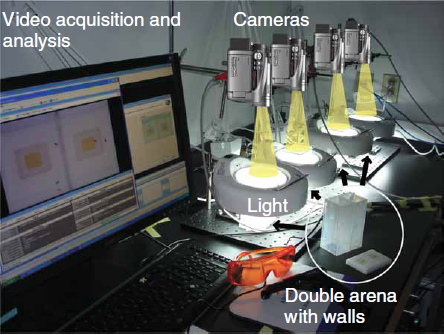
\includegraphics[width=0.35\textwidth]{automated_arena}
}
\subcaptionbox{果蝇活动台尺寸和形状\label{fig:dankert_fly_arena}} {
    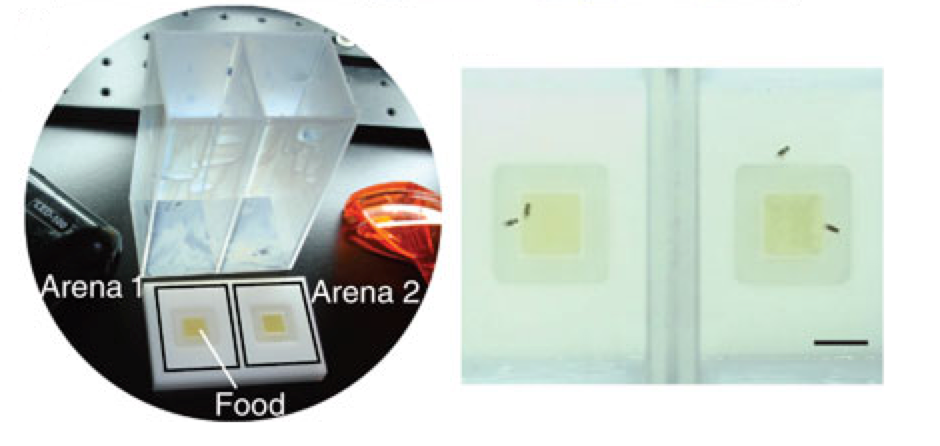
\includegraphics[width=0.55\textwidth]{dankert_arenas}
}
\caption{Dankert的果蝇识别系统的实验环境\cite{dankert2009automated}}\label{fig:dankert_system}
\end{figure}

\begin{figure}
\centering
\subcaptionbox{果蝇拍摄环境\label{fig:raoyi_fly_env}} {
    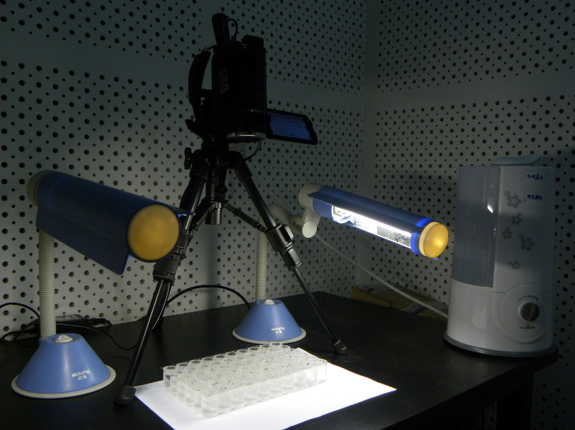
\includegraphics[width=0.5\textwidth]{video_environment}
}
\subcaptionbox{果蝇活动台尺寸和形状\label{fig:raoyi_fly_arena}} {
    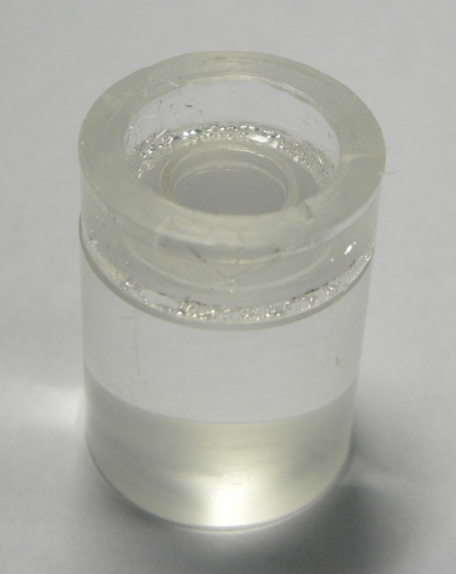
\includegraphics[width=0.3\textwidth]{video_arena}
}
\caption{饶毅实验室果蝇识别系统的实验环境}\label{fig:raoyi_system}
\end{figure}

\section{研究现状}

关于动物行为学的研究早在17、18世纪就已经开始,而随着计算机运算能力的提升、计算机视觉技术的发展,以及机器学习的日益发展,计算机被越来越多的应用到动物行为分析中,包括对果蝇、小鼠、蜜蜂等小动物的研究\cite{physic_mice_2012,marked_mice_2013,veeraraghavan2008shape,JAABA_2013,EthoVision_2001}。目前,在国内外都存在一些科研单位研究果蝇行为学,比如,国内有南京农业大学的梁敬东实验室对果蝇求偶行为的自动化分析\cite{孙吉祥2015基于图像分割和轮廓矩的果蝇求偶行为识别方法,梁敬东2011果蝇求偶行为计算机检测识别方法,谢忠红2016基于视频的果蝇求偶行为识别和运动轨迹跟踪预测,孙吉祥2014果蝇求偶行为的图像识别算法研究,谢元澄2011基于特征选择集成学习的果蝇求偶行为识别}等,北京大学饶毅实验室及其合作单位对果蝇打架行为和求偶行为的自动化分析的相关研究\cite{chexiangqian}。国际上,包括加州理工学院的Dankert、Liming Wang等在特定场景下对果蝇的打架和求偶行为开发了一套果蝇行为自动分析系统,并给出了详细的实施准则\cite{dankert2009automated};哈佛医学院神经生物学系的Selby Chen等设计了一套果蝇打架检测系统,用于帮助对果蝇攻击性行为的研究\cite{3D_fly_2009}。下面,本节将简要介绍动物行为识别中的技术发展概要,重点介绍果蝇行为识别中关键技术的发展,以及果蝇身体轮廓提取的研究现状。

\subsection{背景模型及其在果蝇身体检测中的应用}

在视频处理技术中,运动目标的检测是一个重要部分。通过背景建模,从视频中分离前景和背景,有广泛的应用场景\cite{fu1981survey}。现有的背景模型大多面向道路交通场景,也可以用于果蝇身体和翅膀的轮廓提取。下面介绍几种常见的背景模型,以及在果蝇轮廓提取中的应用。

运动目标检测视频中,当拍摄角度、方位不变时,视频的视野基本固定,可以采用中值滤波、均值滤波等算法\cite{cucchiara2003detecting}进行背景建模。以若干视频帧的中值或均值作为背景。对于实时监测场景,可以将前$K$帧视频的均值或中值图像作为第$K+1$帧的背景。中值滤波、均值滤波算法会受到前景的影响,但是实现比较简单,应用也比较广泛。

帧差法是另一种广泛应用的建模方法。帧差法通过对相邻两帧之间进行做差分,并对差值进行阈值化,保留其中变化较小的部分作为背景。通过改进帧差法,Zhang, HAO分别提出三帧差分法、五帧差分法等\cite{zhang2012three, hao2012moving}。帧差法计算相对简单,对于运动目标的轮廓检测效果好,但是对于物体内部可能出现漏检。

此外,有研究通过统计模型建立背景模型。Elgammal提出一种核密度估计模型\cite{elgammal2002background},假设像素点的分布符从某概率分布,通过对若干视频帧进行统计分析,计算概率分布的参数;根据概率分布模型的参数,判定视频帧中的像素属于前景还是背景。

此外,比较经典的还有单高斯模型、混合高斯模型等\cite{gaussian_1997,power2002understanding,zivkovic2004improved}。单高斯模型主要对背景直接进行建模,不考虑前景的影响。而混合高斯模型通过估计前景和背景的分布,同事对前景和背景进行建模。通过高斯模型,可以分离视频帧中的背景和前景目标。上述高斯模型一般适用于图像变化比较缓慢的场景,在图像变化较快时,效果并不理想。滑动高斯模型对每个像素建立多个高斯模型\cite{martel2005moving},提高了对变化场景的检测能力,但同时也增加了模型的计算量。

Horprasert提出了一种基于颜色信息的背景建模算法\cite{shadow_2000},该算法将彩色空间中视频帧之间的差异分解为亮度差异和色域差异,通过定义亮度畸变,算法可以检测视频帧中前景物体的阴影部分,解决了视频帧中存在阴影问题。此外,算法的复杂度相对不高,检测效果也比较理想。该算法被车向前应用于果蝇身体检测模型中\cite{chexiangqian}。

目前,针对果蝇行为视频而设计的背景模型相对较少。和一般的运动目标检测任务相比,果蝇视频的背景模型具有一些共同点,如,前景物体在背景中不停的运动;但也存在一定的特殊性,包括:果蝇拍摄环境相对简单,受到光照、天气等的影响相对较小,这是有利条件;但是果蝇行为视频的背景模型对准确性要求更高。果蝇轮廓提取一般包括两部分:果蝇身体和果蝇翅膀。果蝇身体区域是决定果蝇特征点的重要依据,果蝇身体区域直接影响包括果蝇的位置、大小、姿态等重要参数,对果蝇特征提取和行为识别有重要影响;果蝇翅膀的行为在果蝇行为学中有明确的意义,比如,打架行为中果蝇通过振翅发出威胁等\cite{fly_fighter_2006}。果蝇身体和果蝇活动台之间存在较大的颜色差异,检测难度相对较低;果蝇翅膀的颜色偏暗,呈现出半透明特点,和果蝇身体、活动台背景很容易混淆,检测起来相对困难。尤其是果蝇翅膀部分对果蝇背景模型提出了很高的要求。

南京林业大学的孙吉祥在论文中提出一种基于直方图统计的背景模型\cite{孙吉祥2014果蝇求偶行为的图像识别算法研究},首先采用OSTU算法计算果蝇身体的轮廓\cite{otsu1975threshold},然后用灰度直方图法,通过求解直方图中的极值点得到视频帧中果蝇身体和果蝇翅膀的阈值,进而实现果蝇身体和翅膀的提取。上述算法计算简单,在视频拍摄条件良好、清晰度较高的情况下可以正常工作,对于视频质量较差的情况,上述算法很难适应。此外,该算法的准确性较差,提取到的果蝇身体轮廓和翅膀轮廓存在明显的噪声。

Dankert在论文的支撑材料中提到了一种背景模型\cite{dankert2009automated},首先求解视频的均值$\mu_I$和方差$\sigma_I^2$,并定义了变量$F_I$用于取代$\mu_I$,作为视频的前景变量:
$$
F_I = 1 - \frac{I}{\mu_I + 3\sigma_I}
$$
论文尝试对$F_I$分别采用混合高斯模型和阈值化进行果蝇轮廓提取\cite{bilmes1998gentle}。其中,混合高斯模型将$F_I$建模为3种不同的高斯分布,分别对应果蝇活动台、果蝇身体和果蝇翅膀部分;阈值化则通过对$F_I$设定阈值,分离果蝇活动台、果蝇身体和果蝇翅膀。经过在300帧的样本上进行实验,最优的阈值化可以取得$96.3\%$的准确率,而混合高斯模型只能取得$59.0\%$的准确率。实验表明,混合高斯模型性能较差,而合适的阈值化虽然简单,却可以得到良好的性能。

车向前采用了单高斯模型\cite{chexiangqian},为了处理果蝇翅膀引入了Horprasert提出的亮度畸变概念\cite{shadow_2000}。此外,车向前还根据果蝇身体的面积,提出了自适应的果蝇轮廓提取算法,取得了较好的效果。但是该算法没有考虑果蝇身体和翅膀对活动台背景的影响,在处理背景亮度不均衡的果蝇行为视频时,会存在一定的误差。

目前,果蝇轮廓提取算法对于拍摄场景的适应性还存在一定的问题,在视频质量较差时,果蝇身体轮廓提取的精确性还有待提高。

\subsection{果蝇行为识别研究分析}

果蝇行为识别一般分为以下几个步骤:果蝇活动台的提取和分割,果蝇轮廓的提取,果蝇特征的提取和果蝇行为的识别。下面分别介绍其研究现状。

关于果蝇活动台分割的研究算法相对比较简单,相关的研究也较少\cite{chexiangqian,dankert2009automated},其方式也基本一致:首先对果蝇活动台进行轮廓提取,然后对轮廓中心进行聚类,得到活动台的中心和大小。目前上述算法的可靠性仍存在一定问题,主要体现在轮廓提取步骤可能找不到合适数目的活动台,以及聚类过程受初始化影响比较严重。

在果蝇行为视频中存在不止一只果蝇,需要对果蝇进行编号。现有的研究一般采用混合高斯模型对果蝇像素点进行聚类,从而划分出果蝇的身体\cite{highThroughput_2009}。Jung提出了一种算法用于分离接触的物体\cite{cell_seg_2010},和直接使用混合高斯模型不同,该算法通过对不同的像素点赋予不同的权重,更好的保持了物体的整体性。上述算法被应用于接触果蝇的身体分割\cite{chexiangqian},取得了良好的效果,但在处理大面积重合的果蝇时,重合部分的处理不尽理想。

在果蝇头部和尾部的判别上,Dankert使用果蝇头部和尾部的灰度信息来判断果蝇的头和尾\cite{dankert2009automated},此外,果蝇的运动方向、视频帧之间的相对位置信息等也可以辅助判断果蝇头部和尾部。


针对果蝇行为识别,目前Dankert使用K最近邻(K-Nearest Neighbor,KNN)算法进行分类\cite{altman1992introduction};车向前使用支持向量机(Support Vector Machine,SVM)对果蝇行为进行分类\cite{chexiangqian,SVM_weight_2004}。但上述算法都没有充分利用到果蝇行为的时间信息。隐马尔科夫模型(Hidden Markov Model, HMM)及其衍生模型能描述状态随时间变化的特点,被应用于各种行为识别领域\cite{baum1966statistical,rabiner1986introduction,ghahramani1997factorial,fine1998hierarchical,blunsom2004hidden},如Brand提出了耦合马尔科夫模型(Coupled Hidden Markov Model, CHMM)\cite{brand1997coupled},用于解决多个个体之间的行为模式分类问题。林国余基于耦合马尔科夫模型提出一种监控镜头中行人异常行为交互识别算法,取得了良好的效果\cite{林国余2013基于耦合隐马尔可夫模型的异常交互行为识别}。

随着深度学习的发展\cite{demuth2014neural,specht1991general},神经网络也被应用于果蝇行为学。在2000年,Gassoumi利用神经网络对昆虫进行分类\cite{gassoumi2000neural},此后,神经网络又被应用于果蝇姿态的识别中。孙吉祥等采用果蝇身体的矩特征作为果蝇身体的特征,并采用神经网络训练果蝇身体的姿态\cite{孙吉祥2014果蝇求偶行为的图像识别算法研究}。除了直接对果蝇姿态进行静态分析,神经网络中的递归神经网络(Recurrent neural network, RNN)和长短期记忆(Long short-term memory,LSTM)等模型也可以用于各种行为检测\cite{mikolov2010recurrent,gers2000learning,veeriah2015differential},朱煜在综述中介绍了深度学习在人体行为识别中的研究进展\cite{朱煜2016基于深度学习的人体行为识别算法综述},W{\"o}llmer提出,利用LSTM模型可以对连续的表情进行识别\cite{wollmer2013lstm},Baccouche使用LSTM对人体行为动作进行识别\cite{baccouche2011sequential}。上述研究有望进一步推广至动物行为学。

\section{研究目标和研究内容}

本文的主要目标在于研究果蝇活动台分割算法和果蝇轮廓提取算法,提升算法的鲁棒性,提升果蝇行为识别算法的应用范围。本文的研究内容主要包括:
\begin{enumerate}
\item 针对现有果蝇活动台提取算法的精确度较低的问题,本文引入了果蝇活动台的排列模式,通过将图像中的活动台和理想排列模式之间建立一一映射,去除果蝇活动台提取过程中的噪声。此外,对于不按照固定模式排列的果蝇活动台,引入自适应机制,减少该步骤中的人工干预;
\item 果蝇行为视频的实验环境和拍摄条件差异给果蝇轮廓提取带来很大的困难,针对此问题,本文提出一种果蝇轮廓提取算法,采用单高斯模型作为背景模型,通过亮度畸变区分果蝇翅膀和身体。初步建模后分离果蝇身体和活动台背景;然后在对活动台单独进建模的基础上,得到精确的背景模型用于轮廓提取。
\item 创建果蝇行为识别网站,对果蝇研究单位提供果蝇视频分析服务。
\end{enumerate}

\section{论文结构和内容概述}

本文剩余部分的结构如下所示:

第2章主要介绍果蝇活动台分割技术。介绍了如何通过调整HoughCircle算法参数,实现果蝇活动台的自适应提取和分割;然后,对基于特定排列的果蝇活动台,介绍通过坐标变换约束实现果蝇活动台位置校准的算法。最后,通过实验证明自适应步骤和排列信息能够提高果蝇活动台分割的性能。

第3章主要介绍果蝇轮廓提取和跟踪技术。首先,介绍一种基于单高斯模型的果蝇轮廓提取算法,然后在单高斯模型的基础上,提出一种针对果蝇活动台的背景模型,最后通过实验证明该模型对不同的视频具有较高的鲁棒性。

第4章主要采用第3章所提的果蝇身体提取算法,并在此基础上实现了果蝇行为识别的完整流程,通过实验给出了果蝇打架行为识别的准确率。实验证明,果蝇行为识别程序可以得到优于人工的识别结果。

第5章主要介绍了果蝇行为识别的网站,首先介绍了果蝇行为识别程序的功能模块、开发和部署环境,然后介绍了网站的基本功能和组成模块,以及其他研究者如何利用网站进行果蝇行为学研究。

第6章对本文工作进行总结,并对将来可能的研究方向进行展望。

